\documentclass[12pt,a4paper]{report}
\usepackage[T1]{fontenc}
\usepackage[utf8]{inputenc}
\usepackage{amsmath,amssymb}
\usepackage{newtxtext,newtxmath}      % Times New Roman text + math
\usepackage[a4paper,margin=1in]{geometry}
\usepackage[protrusion=true,expansion=false]{microtype}  % cleaner justification
\setlength{\emergencystretch}{3em}    % avoid overfull lines
\usepackage{graphicx}
\usepackage{xcolor}
\usepackage{array}
\usepackage{booktabs}
\usepackage{xltabular}                % full-width, page-breakable tables
\usepackage{float}
\usepackage{caption}
\usepackage{enumitem}
\usepackage{setspace}
\usepackage{listings}
\usepackage{chngcntr}                 % \counterwithin on older TeX
\usepackage{tikz}
\usetikzlibrary{arrows.meta,positioning,calc,shapes.geometric}
\usepackage{adjustbox}                % max width=\textwidth for diagrams
\usepackage{titlesec}
\usepackage{titletoc}
\usepackage[hidelinks]{hyperref}

% ---- line spacing 1.15 (Word "line 276 auto") ----
\setstretch{1.15}

% ---- paragraph style: no indent, 6pt gap (matches the template) ----
\setlength{\parindent}{0pt}
\setlength{\parskip}{6pt plus 2pt minus 1pt}

% ---- chapter-relative numbering for tables and figures (Table 2.1, Fig 3.1) ----
\counterwithin{table}{chapter}
\counterwithin{figure}{chapter}
\setcounter{secnumdepth}{3}
\setcounter{tocdepth}{3}

% ---- table column spacing ----
\setlength{\tabcolsep}{5pt}
\newcolumntype{Y}{>{\raggedright\arraybackslash}X}

% ---- heading formats matching the guideline (Times, exact sizes) ----
% CHAPTER n: TITLE  -> 16pt bold, centered
\titleformat{\chapter}[block]
  {\centering\bfseries\fontsize{16}{19}\selectfont}
  {CHAPTER \thechapter:}{0.5em}{}
\titlespacing*{\chapter}{0pt}{8pt}{14pt}
% sections / subsections -> 12pt bold (same size as body, exactly like the guideline)
\titleformat{\section}
  {\bfseries\fontsize{12}{14.5}\selectfont}{\thesection}{0.6em}{}
\titlespacing*{\section}{0pt}{10pt}{4pt}
\titleformat{\subsection}
  {\bfseries\fontsize{12}{14.5}\selectfont}{\thesubsection}{0.6em}{}
\titlespacing*{\subsection}{0pt}{8pt}{3pt}

% ---- TOC chapter entries shown as "CHAPTER n: TITLE" ----
\titlecontents{chapter}[0pt]{\vspace{4pt}\bfseries}
  {CHAPTER \thecontentslabel:\ }{}{\titlerule*[0.6pc]{.}\contentspage}

% ---- monospace listing style for pseudocode / UI wireframes ----
\lstset{
  basicstyle=\ttfamily\footnotesize,
  columns=fixed,
  keepspaces=true,
  breaklines=true,
  breakatwhitespace=true,
  frame=single,
  rulecolor=\color{gray!50},
  framesep=4pt,
  xleftmargin=4pt,
  aboveskip=6pt, belowskip=6pt,
}

\captionsetup{font=small,labelfont=bf}

% ---- TikZ diagram styles ----
\tikzset{
  blk/.style={rectangle, draw, rounded corners=1.5pt, align=center,
              font=\small, inner sep=4pt, minimum height=8mm, fill=black!4},
  tier/.style={rectangle, draw, align=center, font=\small, inner sep=6pt,
               minimum height=12mm, fill=black!4, rounded corners=2pt},
  ent/.style={rectangle, draw, align=center, font=\footnotesize\ttfamily,
              inner sep=3pt, fill=blue!6, minimum height=6mm, minimum width=15mm},
  assoc/.style={rectangle, draw, align=center, font=\footnotesize\ttfamily,
                inner sep=3pt, fill=orange!12, minimum height=6mm},
  proc/.style={ellipse, draw, align=center, font=\footnotesize, inner sep=2pt,
               fill=black!5, minimum width=18mm, minimum height=10mm},
  store/.style={rectangle, draw, align=center, font=\footnotesize, fill=yellow!15,
                minimum height=7mm, inner sep=3pt},
  ext/.style={rectangle, draw, thick, align=center, font=\footnotesize,
              fill=green!8, minimum height=8mm, inner sep=3pt},
  fl/.style={-{Stealth[length=2mm]}, semithick},
  bi/.style={{Stealth[length=2mm]}-{Stealth[length=2mm]}, semithick},
  lbl/.style={font=\scriptsize, inner sep=1pt},
  card/.style={font=\scriptsize, fill=white, inner sep=1.2pt},
}

\begin{document}
\pagenumbering{roman}

\begin{titlepage}
\centering
\vspace*{0.3in}
\IfFileExists{media/image1.png}{
\includegraphics[width=4.02in]{media/image1.png}\par\vspace{0.3in}}{}
{\fontsize{19.5}{23}\selectfont\bfseries HELIX\par}
\vspace{6pt}
{\fontsize{15.5}{19}\selectfont\bfseries A Multi-Tenant Collaborative AI Workspace with Branchable\\
Conversations and a Monitored Deep-Reasoning Mode\par}
\vspace{0.35in}
{\fontsize{15.5}{19}\selectfont by\par}
\vspace{8pt}
{\fontsize{13}{16}\selectfont\bfseries Achindra Sharma (2547105)\\[2pt]
Rajnish Kumar (2547143)\\[2pt]
M M Mohamed Mansoor (2547132)\par}
\vspace{0.3in}
{\fontsize{13}{16}\selectfont Under the guidance of\par}
\vspace{4pt}
{\fontsize{13}{16}\selectfont\bfseries <Guide Name>\par}
\vspace{0.35in}
{\fontsize{12}{15}\selectfont Specialization Project report submitted in partial fulfillment of\\
the requirements of IV trimester MCA,\par}
\vspace{4pt}
{\fontsize{12}{15}\selectfont\bfseries CHRIST (Deemed to be University)\par}
\vspace{0.3in}
{\fontsize{15.5}{19}\selectfont\bfseries August 2026\par}
\end{titlepage}

\thispagestyle{plain}
\begin{center}{\fontsize{16}{19}\selectfont\bfseries\underline{CERTIFICATE}}\end{center}
\addcontentsline{toc}{chapter}{CERTIFICATE}

This is to certify that the report titled ``Helix --- A Multi-Tenant Collaborative AI Workspace with Branchable Conversations and a Monitored Deep-Reasoning Mode'' is a bona fide record of work done by Achindra Sharma (2547105), Rajnish Kumar (2547143) and M M Mohamed Mansoor (2547132), of CHRIST (Deemed to be University), Bangalore, in partial fulfillment of the requirements of IV Trimester MCA during the year 2026.

\vspace{0.5in}

\noindent\textbf{Project Guide}\hfill\textbf{Head of the Department}
\vspace{0.4in}

Valued by:

Name :

Register Number :

Examination Centre : CHRIST (Deemed to be University)

Date of Exam :

\clearpage
\begin{center}{\fontsize{16}{19}\selectfont\bfseries ACKNOWLEDGEMENTS}\end{center}
\addcontentsline{toc}{chapter}{ACKNOWLEDGEMENTS}

We express our sincere gratitude to our project guide for the continued guidance and encouragement throughout the development of Helix. We thank the Department of Computer Science, CHRIST (Deemed to be University), for providing the resources and the academic environment that made this work possible, and our families and peers for their constant support.

\clearpage
\begin{center}{\fontsize{16}{19}\selectfont\bfseries ABSTRACT}\end{center}
\addcontentsline{toc}{chapter}{ABSTRACT}

Teams increasingly use AI for knowledge work, but today's AI tools are built for one person in one private tab. As a result, teammates run prompts in isolation, cannot see or continue each other's conversations, and keep no record of what has already been tried --- causing duplicated effort, wasted API budget, and lost progress.

Helix is a multi-tenant collaborative AI workspace that addresses this gap. A team shares one workspace where conversations can be shared or private, any thread can be forked and branched to explore alternatives, and a shared prompt library captures what works. Live updates and presence make the workspace feel shared. For hard, open-ended problems, any conversation can be escalated into a Deep Reasoning mode --- a recursive reasoning run the whole team can watch live, with a kill switch, a steer/pause control, and a cost-budget meter so a long autonomous run never becomes an opaque, runaway black box. Helix is model-agnostic, running on either hosted (Groq) or local (Ollama) LLMs, so teams can adopt it on their own terms. The project demonstrates three core technical concepts --- Agentic AI (the recursive engine), Distributed Systems (real-time multi-client synchronisation), and Security/RBAC (strict multi-tenancy with a per-action permission policy).

\clearpage
\renewcommand{\contentsname}{\centerline{\normalfont\bfseries\fontsize{16}{19}\selectfont TABLE OF CONTENTS}}
\renewcommand{\listfigurename}{\centerline{\normalfont\bfseries\fontsize{16}{19}\selectfont LIST OF FIGURES}}
\renewcommand{\listtablename}{\centerline{\normalfont\bfseries\fontsize{16}{19}\selectfont LIST OF TABLES}}
\tableofcontents
\clearpage
\listoffigures
\clearpage
\listoftables
\clearpage
\pagenumbering{arabic}

\chapter{INTRODUCTION}
This chapter introduces the project, the motivation and problem it addresses, its objectives, related existing works, the expected benefits, the project's purpose, scope and applicability, and the plan of work.

\section{Background and Motivation}
AI assistants such as ChatGPT, Claude, Gemini, and locally run open models have become a routine part of how engineering teams, student project groups, and research teams do knowledge work --- but the tools have not caught up to the fact that this work is collaborative. Knowledge gained in one person's session is invisible to everyone else; the same prompts get re-written from scratch; and when a teammate is away, nobody can pick up their thread. As teams begin using AI for longer, more autonomous reasoning, a second gap appears: those runs are opaque and can quietly burn time and budget.

The motivation for Helix is to make team AI work shared, reusable, and --- when it gets ambitious --- observable and controllable. By capping and controlling long autonomous runs and eliminating duplicated compute, the project also aligns with Sustainable Development Goal 12 (Responsible Consumption and Production).

\section{Problem Statement}
When teams do knowledge work with AI together, three problems follow:

\begin{enumerate}
  \item Siloed context --- Teammates cannot see each other's conversations or reuse what has already been tried, causing redundant queries, wasted budget, and lost progress when someone needs to pick up where a colleague left off.
  \item No branching --- Linear chats cannot fork, so a promising thread cannot be cloned to explore an alternative without disrupting the original.
  \item Unmonitored autonomy --- Long, autonomous AI runs are opaque: no mid-run visibility, no stop control, and no cost guardrail --- risking wasted compute and runaway cost before anyone can intervene.
\end{enumerate}

\section{Objectives}
\begin{enumerate}
  \item Provide multi-tenant workspaces with accounts, invite-link onboarding, and roles (Owner / Collaborator / Observer), with strict per-tenant isolation.
  \item Support shared and private conversations within a workspace.
  \item Deliver real-time sync and presence so members see updates and streaming responses live.
  \item Implement fork and branch of any conversation as a persistent tree.
  \item Build a shared prompt library with tags and search to capture reusable prompts.
  \item Provide a Deep Reasoning mode: an escalation into a recursive reasoning run.
  \item Provide a monitor for Deep Reasoning runs --- live trace, kill switch, steer/pause, and a token/cost budget meter.
  \item Persist conversations and runs for replay and export (JSON / Markdown).
  \item Remain model-agnostic and cost-aware --- runnable on hosted or local LLMs, with explicit controls on long-run token spend.
\end{enumerate}

\section{Existing Works}
Each existing category solves only one slice of collaborative AI work; Helix's contribution is the combination of shared and branchable conversations, a reusable prompt library, and a monitored deep-reasoning mode in one workspace.

\begingroup
\setlength{\parskip}{0pt}\renewcommand{\arraystretch}{1.32}\footnotesize
\begin{xltabular}{\textwidth}{>{\hsize=0.8571\hsize\raggedright\arraybackslash}X >{\hsize=0.8571\hsize\raggedright\arraybackslash}X >{\hsize=1.2857\hsize\raggedright\arraybackslash}X}
\caption{Existing works and the gap Helix fills}\\
\toprule
\textbf{System} & \textbf{Strength} & \textbf{Gap Helix fills} \\
\midrule\endfirsthead
\toprule
\textbf{System} & \textbf{Strength} & \textbf{Gap Helix fills} \\
\midrule\endhead
\bottomrule\endfoot
ChatGPT / Claude (web) & Strong single-user chat & One person, one tab --- no sharing, branching, or library \\
ChatGPT Team / Claude Projects & Shared files \& history & Asynchronous sharing only --- no live branchable conversations or reusable prompt library \\
Prompt managers (e.g. PromptHub) & Prompt storage & Standalone --- not tied to live team conversations or reasoning \\
Agent frameworks (LangGraph, etc.) & Agent orchestration & Single-developer; no collaboration, no monitoring/kill switch out of the box \\
\end{xltabular}
\endgroup

\section{Benefits of the Proposed Work}
\begin{itemize}
  \item No duplicated effort --- shared conversations and a prompt library mean the team reuses what works instead of re-asking.
  \item Continuity --- anyone can pick up where a teammate left off.
  \item Parallel exploration --- branching lets the team try competing approaches without losing context.
  \item Cost and oversight --- the monitor caps and controls long autonomous runs, cutting wasted compute (SDG 12).
  \item Flexible deployment --- model-agnostic, running on hosted or local LLMs, so teams choose by cost, privacy, or latency.
\end{itemize}

\section{Purpose, Scope and Applicability}
\subsection{Purpose}
The purpose of Helix is to remove the black boxes from team AI work --- to make a team's reasoning shared, branchable, reusable and, for autonomous runs, observable and controllable. It improves the current way of working by replacing isolated private tabs with one shared, recorded workspace, and by replacing opaque autonomous runs with a governed, watchable one.

\subsection{Scope}
The project delivers a working multi-tenant web application: authentication and workspaces, shared/private conversations with real-time sync, fork-and-branch, a shared prompt library, a Deep Reasoning mode with a live monitor (kill / steer / budget), and history replay and export. It assumes a small team per workspace and a single backend instance for the core demonstration (horizontal scaling via Redis pub/sub is an optional extension). Inference runs through a pluggable provider on either hosted (Groq) or local (Ollama) models.

\subsection{Applicability}
Helix is directly applicable to software engineering teams, student project groups, and research teams that use AI collaboratively. Indirectly, by capping and controlling autonomous runs it contributes to responsible, cost-aware use of compute, and by being model-agnostic it supports privacy-sensitive deployments on fully local models.

\section{Plan of Work}
The work spans approximately twelve weeks (2 June 2026 -- 25 August 2026) across a team of three. The collaborative core is built first on plain chat, after which the Deep Reasoning mode and its monitor are added. Responsibility is split as: Achindra Sharma --- Deep Reasoning engine and integration; Rajnish Kumar --- backend and infrastructure; M M Mohamed Mansoor --- frontend and UX (roles may be adjusted by mutual agreement).

\begingroup
\setlength{\parskip}{0pt}\renewcommand{\arraystretch}{1.32}\footnotesize
\begin{xltabular}{\textwidth}{>{\hsize=1.6200\hsize\raggedright\arraybackslash}X >{\hsize=0.7500\hsize\raggedright\arraybackslash}X >{\hsize=0.6300\hsize\raggedright\arraybackslash}X}
\caption{Plan of Work}\\
\toprule
\textbf{Task / Module} & \textbf{Person Responsible} & \textbf{Duration} \\
\midrule\endfirsthead
\toprule
\textbf{Task / Module} & \textbf{Person Responsible} & \textbf{Duration} \\
\midrule\endhead
\bottomrule\endfoot
Project setup --- monorepo, Docker Compose (Postgres / Redis / Ollama), shared schemas & All & 02 Jun -- 08 Jun \\
M1 --- Auth \& Workspace (accounts, JWT, workspaces, invite links, roles, DB schema) & Rajnish Kumar & 09 Jun -- 22 Jun \\
M2 --- Conversations (provider interface Groq/Ollama; shared \& private conversations; streaming chat) & Achindra Sharma & 09 Jun -- 22 Jun \\
Auth \& workspace UI (login/register, workspace dashboard, chat view) & M M Mohamed Mansoor & 09 Jun -- 22 Jun \\
M3 --- Real-Time Sync \& Presence (WebSocket rooms, presence, ordered message log) & Rajnish Kumar & 23 Jun -- 06 Jul \\
Shared context (append to shared thread, token budgeting, summarisation) & Achindra Sharma & 23 Jun -- 06 Jul \\
Collaboration UI (multi-user shared view, presence avatars, stream fan-out) & M M Mohamed Mansoor & 23 Jun -- 06 Jul \\
M4 --- Fork \& Branch Tree (fork via parent pointers; branch context) & Achindra Sharma / Rajnish Kumar & 07 Jul -- 13 Jul \\
M5 --- Shared Prompt Library (save / tag / search prompts; reuse) & M M Mohamed Mansoor & 14 Jul -- 20 Jul \\
M6 --- Deep Reasoning Mode (recursive engine; escalation path; checkpoint fork) & Achindra Sharma & 21 Jul -- 03 Aug \\
M7 --- Monitor (backend): persist runs/steps, stream events, kill/steer endpoints, budget metering & Rajnish Kumar & 21 Jul -- 10 Aug \\
M7 --- Monitor (UI): Deep Reasoning button, live trace/topology, kill switch, steer, budget meter & M M Mohamed Mansoor & 28 Jul -- 10 Aug \\
M8 --- History, Replay \& Export (replay any branch; JSON/Markdown export) & Achindra Sharma & 11 Aug -- 17 Aug \\
M9 --- Permission Layer (role-gated actions; tool allowlist for Deep Reasoning) & Rajnish Kumar & 11 Aug -- 17 Aug \\
Hardening \& demo (tenant isolation/RLS, deployment, performance test, demo video, README) & All & 18 Aug -- 25 Aug \\
\end{xltabular}
\endgroup

\section{Overview of the Report}
The remainder of this report is organised as follows. Chapter 2 --- System Analysis and Requirements --- studies the existing systems and their limitations, defines the proposed system, its benefits and features, and specifies the functional, non-functional, software and hardware requirements. Chapter 3 --- System Design --- presents the system architecture, module design, data-flow and ER diagrams, database design, user-interface design, and the algorithm design for the core mechanisms of Helix.

\chapter{SYSTEM ANALYSIS AND REQUIREMENTS}
This chapter studies the existing systems and their limitations, defines the proposed system with its benefits and features, and specifies the system requirements.

\section{Existing System}
AI assistants such as ChatGPT, Claude, Gemini, and locally run open models have become a routine part of team knowledge work, yet almost every mainstream tool is built around a single assumption: one user, one private conversation. Studying how teams actually use these tools reveals five distinct categories of existing system, each solving only one slice of collaborative AI work.

\begingroup
\setlength{\parskip}{0pt}\renewcommand{\arraystretch}{1.32}\footnotesize
\begin{xltabular}{\textwidth}{>{\hsize=0.2925\hsize\raggedright\arraybackslash}X >{\hsize=1.0512\hsize\raggedright\arraybackslash}X >{\hsize=1.2340\hsize\raggedright\arraybackslash}X >{\hsize=1.3711\hsize\raggedright\arraybackslash}X >{\hsize=1.0512\hsize\raggedright\arraybackslash}X}
\caption{Categories of existing systems}\\
\toprule
\textbf{\#} & \textbf{Category} & \textbf{Representative tools} & \textbf{What it does well} & \textbf{The slice it owns} \\
\midrule\endfirsthead
\toprule
\textbf{\#} & \textbf{Category} & \textbf{Representative tools} & \textbf{What it does well} & \textbf{The slice it owns} \\
\midrule\endhead
\bottomrule\endfoot
1 & Single-user chat assistants & ChatGPT, Claude.ai, Gemini & Fast, high-quality single-user question answering & The conversation itself \\
2 & Team AI suites & ChatGPT Team, Claude Projects / Teams & Shared files, shared history, seat \& billing management & Sharing artifacts and history \\
3 & Prompt managers & PromptLayer, ad-hoc notebooks / spreadsheets & Storing and organising prompts & The record of prompts \\
4 & Agent frameworks & LangChain, LangGraph, AutoGPT, CrewAI & Orchestrating autonomous multi-step agents & The reasoning loop \\
5 & Agent observability & LangSmith, Langfuse, Helicone & Tracing \& monitoring agent runs after they finish & Visibility into runs \\
\end{xltabular}
\endgroup

When a team faces a hard, open-ended problem, the work fragments without anyone deciding it should: members open parallel private tabs that none of the others can see; useful fragments are copy-pasted into a chat channel stripped of their surrounding context; trying a different angle means overwriting or restarting a thread and losing the original line of thought; a carefully crafted prompt that worked last week lives in one person's history and is rewritten from scratch by the next person; and for genuinely hard questions a member might wire up an agent framework locally whose run is invisible and uncontrollable to the rest of the team.

No single existing system combines all four of the capabilities a collaborating team needs at once: a shared, live conversation surface; branchable threads that preserve lineage; a reusable, searchable prompt record; and a governed, watchable autonomous reasoning mode. Helix exists to close those seams in one product.

\section{Limitations of the Existing System}
The study above translates into seven concrete limitations that the proposed system must overcome.

\begin{itemize}
  \item L1 --- Isolation and siloed context. Conversations are private by default; a colleague cannot see, continue, or learn from another member's thread, so the team repeatedly re-asks questions already answered.
  \item L2 --- No branching; lossy exploration. Mainstream chat tools present a single linear thread, and editing an earlier message destroys the alternative rather than preserving it.
  \item L3 --- No shared, reusable prompt record. Working prompts are trapped in one person's history or informal documents; there is no workspace-scoped, tagged, searchable library.
  \item L4 --- Autonomy without governance. Where agent frameworks offer multi-step autonomous reasoning, the run is a black box: no live trace, no kill switch, no mid-flight steer, and no cost ceiling.
  \item L5 --- Weak team and tenancy model. Single-user tools have no workspace roles; team suites add seats but not fine-grained, per-action permissions.
  \item L6 --- Observability is post-hoc and separate. Observability tools trace runs after they complete, inside a different product, with no in-the-moment control.
  \item L7 --- Lock-in and cost. Most team AI is billed per seat or per token against a single hosted provider, with no model-agnostic local option.
\end{itemize}

\section{Proposed System}
The core problem is that collaborative AI work is forced through single-user tools, so context is siloed, exploration is lossy, prompts are not reused, and autonomous runs are ungoverned. Helix decomposes this into sub-problems --- tenancy and access (L5), shared and private conversations (L1), branching (L2), prompt reuse (L3), real-time collaboration (L1, L6), governed autonomous reasoning (L4, L6), and model flexibility (L7) --- and solves each as a feature of one product.

Helix is a multi-tenant collaborative AI workspace --- informally, ``Git for your team's AI work.'' Instead of everyone prompting alone in private tabs, a team shares one workspace where AI conversations are shared, branchable, recorded, and --- when a problem is hard enough --- escalated into a monitored deep-reasoning run.

\section{Benefits of the Proposed System}
\begin{itemize}
  \item Eliminates duplicated effort through shared conversations and a reusable prompt library.
  \item Provides continuity --- any member can resume a teammate's thread.
  \item Enables parallel exploration via O(1) forking that preserves lineage.
  \item Governs cost and autonomy through a live monitor with kill switch, steer/pause and a budget meter (SDG 12).
  \item Offers flexible, model-agnostic deployment on hosted (Groq) or local (Ollama) models.
\end{itemize}

\section{Features of the Proposed System}
Each feature directly answers one or more of the limitations identified in Section 2.2.

\begingroup
\setlength{\parskip}{0pt}\renewcommand{\arraystretch}{1.32}\footnotesize
\begin{xltabular}{\textwidth}{>{\hsize=0.9600\hsize\raggedright\arraybackslash}X >{\hsize=0.3300\hsize\raggedright\arraybackslash}X >{\hsize=1.7100\hsize\raggedright\arraybackslash}X}
\caption{Features of the proposed system}\\
\toprule
\textbf{Feature} & \textbf{Answers} & \textbf{Description} \\
\midrule\endfirsthead
\toprule
\textbf{Feature} & \textbf{Answers} & \textbf{Description} \\
\midrule\endhead
\bottomrule\endfoot
F1 --- Multi-tenant workspaces with RBAC & L5 & Authenticated accounts, invite-link onboarding, three roles (Owner/Collaborator/Observer); every resource scoped to one isolated workspace tenant. \\
F2 --- Shared and private conversations & L1 & A conversation belongs to a workspace and is shared or private; AI responses stream token-by-token. Shared conversations become durable team knowledge. \\
F3 --- Fork and branch tree & L2 & Any conversation can be forked into an independent branch that inherits parent context but evolves separately, visualised as a persistent Git-style tree. Forking copies no history. \\
F4 --- Shared prompt library & L3 & Working prompts are saved with tags and full-text search, and can be inserted into any conversation for reuse. \\
F5 --- Real-time collaboration and presence & L1, L6 & A live channel per workspace broadcasts new messages, streaming tokens, and presence signals. \\
F6 --- Deep Reasoning mode & L4 & A hard question can be escalated into a recursive engine that reasons, reflects on its own thinking, and synthesises --- looping until it converges. \\
F7 --- Monitor and run control & L4, L6 & A live monitor with a reasoning trace and topology view, a kill switch, a steer/pause control, a recursion-depth guard, and a token-cost budget meter with alerts. \\
F8 --- Model-agnostic provider layer & L7 & All inference flows through one provider interface with interchangeable hosted (Groq) and local (Ollama) backends, selected by configuration. \\
F9 --- History, replay, and export & L1, L6 & Conversations and runs are persisted; any branch can be replayed step by step and exported as JSON or Markdown. \\
\end{xltabular}
\endgroup

Together these features demonstrate the project's three core technical concepts: Agentic AI (the recursive Deep Reasoning engine), Distributed Systems (real-time multi-client synchronisation, ordering, and fan-out), and Security / RBAC (strict multi-tenancy with a per-action permission policy).

\section{System Requirements Specification}
This section defines the requirements of the system without focusing on how they will be achieved.

\subsection{User Characteristics}
Helix serves three kinds of user, distinguished by role within a workspace:

\begin{itemize}
  \item Owner --- creates the workspace, invites and manages members and roles, edits the permission policy, and has full authority over conversations and runs.
  \item Collaborator --- a working member who can send messages, fork conversations, save and use library prompts, escalate to Deep Reasoning, and steer or kill runs.
  \item Observer --- a read-only member who can view, replay and export conversations and watch Deep Reasoning runs, but cannot act on them.
\end{itemize}

\subsection{Software and Hardware Requirements}
\noindent\textbf{(i) Software Requirements}

\begingroup
\setlength{\parskip}{0pt}\renewcommand{\arraystretch}{1.32}\footnotesize
\begin{xltabular}{\textwidth}{>{\hsize=0.5946\hsize\raggedright\arraybackslash}X >{\hsize=1.4054\hsize\raggedright\arraybackslash}X}
\caption{Software requirements}\\
\toprule
\textbf{Category} & \textbf{Requirement} \\
\midrule\endfirsthead
\toprule
\textbf{Category} & \textbf{Requirement} \\
\midrule\endhead
\bottomrule\endfoot
Operating System & Cross-platform; Linux containers for deployment \\
Frontend & React, TypeScript, TailwindCSS, Vite; modern browser \\
Backend & Python 3.11+, FastAPI, WebSockets \\
Deep Reasoning engine & LangGraph (recursive reasoning, checkpointing) \\
LLM inference & Pluggable provider --- Groq (hosted) or Ollama (local), via an OpenAI-compatible interface \\
Database & PostgreSQL (production) / SQLite (development) \\
Containerisation & Docker + Docker Compose (local development) \\
Version control & Git / GitHub \\
Optional (scaling only) & Redis --- pub/sub fan-out across multiple backend instances \\
\end{xltabular}
\endgroup

\noindent\textbf{(ii) Hardware Requirements}

\begingroup
\setlength{\parskip}{0pt}\renewcommand{\arraystretch}{1.32}\footnotesize
\begin{xltabular}{\textwidth}{>{\hsize=0.6383\hsize\raggedright\arraybackslash}X >{\hsize=1.0851\hsize\raggedright\arraybackslash}X >{\hsize=1.2766\hsize\raggedright\arraybackslash}X}
\caption{Hardware requirements}\\
\toprule
\textbf{Component} & \textbf{Minimum (development)} & \textbf{Notes} \\
\midrule\endfirsthead
\toprule
\textbf{Component} & \textbf{Minimum (development)} & \textbf{Notes} \\
\midrule\endhead
\bottomrule\endfoot
CPU & Quad-core x86-64 & Backend, DB, containers \\
RAM & 8 GB (16 GB recommended) & \textasciitilde{}8 GB if running local Ollama; otherwise use Groq \\
Storage & 10 GB free & Docker images, DB, optional model weights \\
Network & Broadband & Required for hosted inference (or run Ollama locally) \\
Client & Any modern desktop/laptop with a browser & No special hardware \\
Deployment & Any container host & No owned servers required \\
\end{xltabular}
\endgroup

\subsection{Constraints}
\begin{itemize}
  \item Hardware limitations --- running a local Ollama model requires roughly 8 GB of RAM; otherwise hosted Groq inference is used.
  \item Language / platform --- Python 3.11+ on the backend, TypeScript/React on the frontend, and a modern browser on the client.
  \item Interfaces to other applications --- LLM access via an OpenAI-compatible interface (Groq / Ollama); persistence via PostgreSQL/SQLite; optional Redis for pub/sub.
  \item Reliability --- every Deep Reasoning run must be haltable at the next step by the kill switch, bounded by recursion-depth, loop and compute-budget guards.
  \item Regulatory / privacy --- only the data needed to operate is collected; no biometric, audio or video data is captured.
\end{itemize}

\subsection{Functional Requirements}
\begingroup
\setlength{\parskip}{0pt}\renewcommand{\arraystretch}{1.32}\footnotesize
\begin{xltabular}{\textwidth}{>{\hsize=0.3173\hsize\raggedright\arraybackslash}X >{\hsize=0.8942\hsize\raggedright\arraybackslash}X >{\hsize=1.7885\hsize\raggedright\arraybackslash}X}
\caption{Functional Requirements}\\
\toprule
\textbf{ID} & \textbf{Requirement} & \textbf{Description} \\
\midrule\endfirsthead
\toprule
\textbf{ID} & \textbf{Requirement} & \textbf{Description} \\
\midrule\endhead
\bottomrule\endfoot
FR-1 & Authentication \& Accounts & Registration and login with hashed credentials; issues signed JWT tokens for REST and real-time endpoints. \\
FR-2 & Workspaces \& Multi-Tenancy & Create workspaces, onboard members via invite links, and scope every resource to one isolated workspace tenant. \\
FR-3 & Role-Based Access Control & Assign each member a role (Owner/Collaborator/Observer) and authorise every action against a role-to-permission policy table. \\
FR-4 & Shared \& Private Conversations & Create shared or private conversations and stream AI responses token-by-token. \\
FR-5 & Real-Time Sync \& Presence & Maintain one real-time room per workspace broadcasting messages, tokens and presence, with a single ordered append-only log. \\
FR-6 & Conversation Fork \& Branch Tree & Fork any conversation at any point into a child branch that inherits context and evolves independently, persisted as a branch tree. \\
FR-7 & Shared Prompt Library & Save prompts with tags to a workspace library, search/browse it, and insert a saved prompt into a conversation. \\
FR-8 & LLM Provider Abstraction & Route all inference through one provider interface with interchangeable Groq/Ollama backends, selectable by configuration. \\
FR-9 & Deep Reasoning Mode & Escalate a conversation into a recursive reason-reflect-synthesize run emitting a structured step event per transition. \\
FR-10 & Deep Reasoning Monitor & A live dashboard consuming step/token events, showing the trace, topology, and energy/depth/loop-guard values in real time. \\
FR-11 & Run Control (Kill \& Steer) & An authorised kill switch halting at the next step boundary, and a steer control that pauses and resumes a run with injected guidance. \\
FR-12 & Budget Meter \& Guardrails & Meter token usage and request rate per workspace against thresholds with alerts, and bound run spend via a compute-budget halt. \\
FR-13 & History, Replay \& Export & Persist conversations and runs, replay any branch step by step, and export as JSON or Markdown. \\
FR-14 & Permission Layer & Owner-restricted tool allowlist for Deep Reasoning and human approval before high-risk tool execution, layered on RBAC. \\
\end{xltabular}
\endgroup

\subsection{Non-Functional Requirements}
\begingroup
\setlength{\parskip}{0pt}\renewcommand{\arraystretch}{1.32}\footnotesize
\begin{xltabular}{\textwidth}{>{\hsize=0.3173\hsize\raggedright\arraybackslash}X >{\hsize=0.8942\hsize\raggedright\arraybackslash}X >{\hsize=1.7885\hsize\raggedright\arraybackslash}X}
\caption{Non-Functional Requirements}\\
\toprule
\textbf{ID} & \textbf{Attribute} & \textbf{Description} \\
\midrule\endfirsthead
\toprule
\textbf{ID} & \textbf{Attribute} & \textbf{Description} \\
\midrule\endhead
\bottomrule\endfoot
NFR-1 & Performance \& Latency & Real-time events (message broadcast, presence, token fan-out) reach clients with a target latency under 200 ms. \\
NFR-2 & Multi-Tenancy \& Isolation & Tenant isolation via workspace-scoped queries and database row-level security; no data crosses tenant boundaries. \\
NFR-3 & Cost Efficiency & Long-run token spend bounded by a compute-budget halt and per-workspace meter; runs on free hosted (Groq) or local (Ollama) models. \\
NFR-4 & Scalability & Single-instance in-memory rooms; optional pub/sub layer for horizontal scaling without session affinity. \\
NFR-5 & Security & All endpoints protected by token auth and RBAC; Deep Reasoning tool use limited to a safe allowlist. \\
NFR-6 & Reliability \& Interruptibility & Any run is haltable at the next step; recursion-depth and compute-budget guards prevent runaway loops; safe error reporting. \\
NFR-7 & Streaming \& Backpressure & A single response stream fans out to many clients without a slow client stalling the others. \\
NFR-8 & Privacy & Only operational data is collected; no biometric, audio, or video data is captured. \\
NFR-9 & Portability & Fully containerisable; the provider interface allows new LLM backends without application changes. \\
\end{xltabular}
\endgroup

\section{Block Diagram}
The block diagram below models the system under study --- the React client, the FastAPI backend (auth/RBAC gate, services, provider layer, sync layer, Deep Reasoning engine) and the relational database --- and the major flows between them (REST/SSE for authoritative reads/writes, WebSocket for presence and broadcast, and the pluggable LLM backend).

\begin{figure}[H]\centering
\begin{adjustbox}{max width=\textwidth}
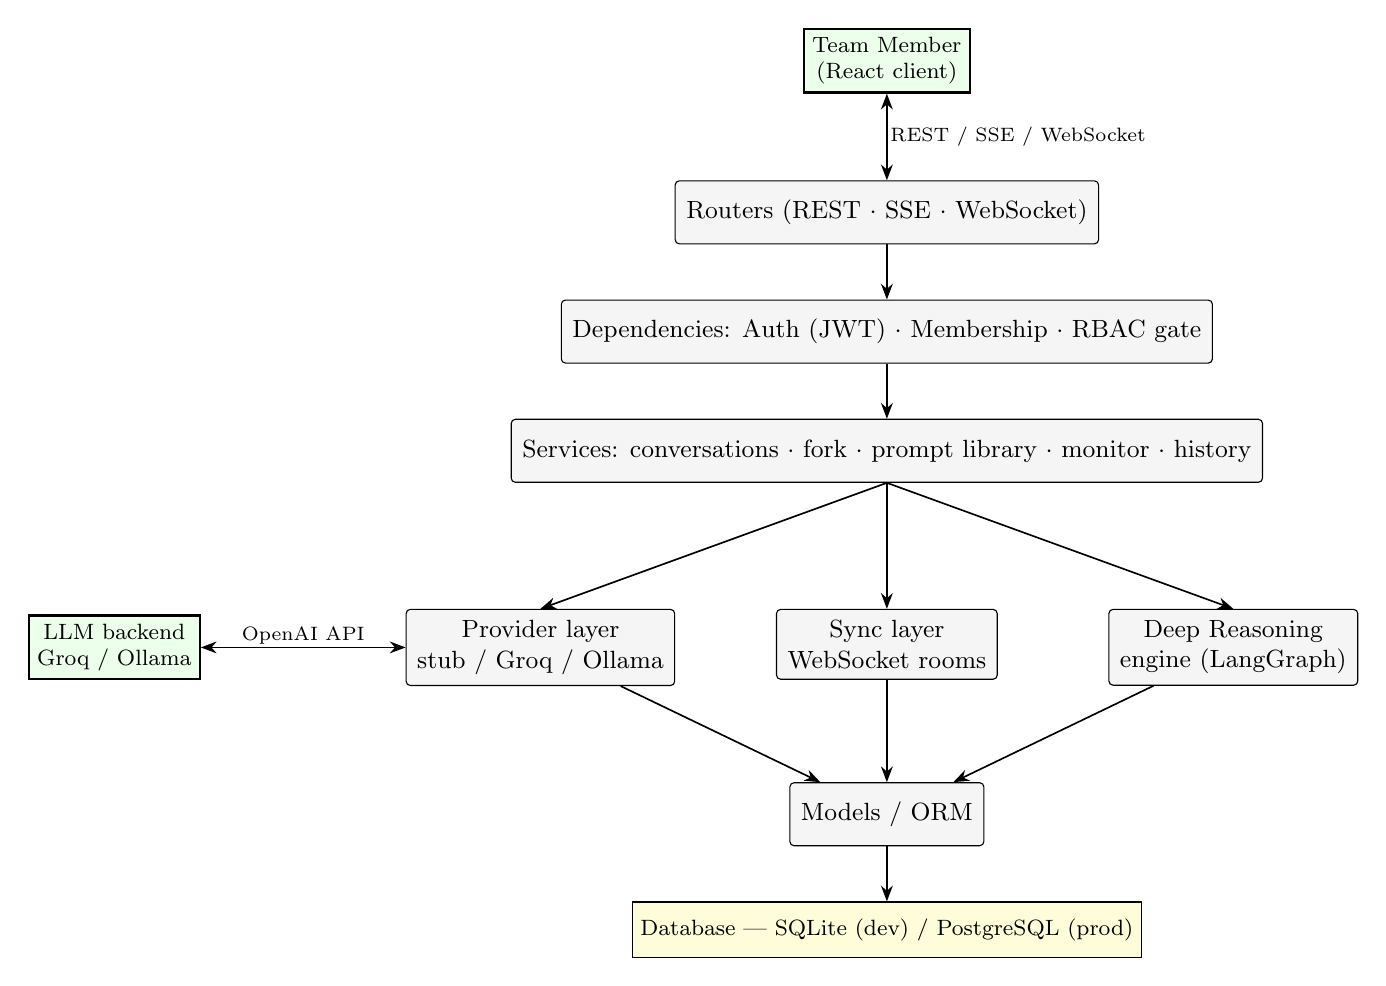
\begin{tikzpicture}
\node[ext] (client) {Team Member\\(React client)};
\node[blk, below=11mm of client] (routers) {Routers (REST $\cdot$ SSE $\cdot$ WebSocket)};
\node[blk, below=7mm of routers] (deps) {Dependencies: Auth (JWT) $\cdot$ Membership $\cdot$ RBAC gate};
\node[blk, below=7mm of deps] (svc) {Services: conversations $\cdot$ fork $\cdot$ prompt library $\cdot$ monitor $\cdot$ history};
\node[blk, below=16mm of svc, xshift=-44mm] (prov) {Provider layer\\stub / Groq / Ollama};
\node[blk, below=16mm of svc] (sync) {Sync layer\\WebSocket rooms};
\node[blk, below=16mm of svc, xshift=44mm] (eng) {Deep Reasoning\\engine (LangGraph)};
\node[blk, below=13mm of sync] (orm) {Models / ORM};
\node[store, below=7mm of orm] (db) {Database --- SQLite (dev) / PostgreSQL (prod)};
\node[ext, left=26mm of prov] (llm) {LLM backend\\Groq / Ollama};
\draw[bi] (client) -- node[lbl,right]{REST / SSE / WebSocket} (routers);
\draw[fl] (routers) -- (deps);
\draw[fl] (deps) -- (svc);
\draw[fl] (svc.south) -- (prov.north);
\draw[fl] (svc.south) -- (sync.north);
\draw[fl] (svc.south) -- (eng.north);
\draw[bi] (prov) -- node[lbl,above]{OpenAI API} (llm);
\draw[fl] (prov) -- (orm);
\draw[fl] (sync) -- (orm);
\draw[fl] (eng) -- (orm);
\draw[fl] (orm) -- (db);
\end{tikzpicture}
\end{adjustbox}
\caption{System block / context diagram of Helix}
\end{figure}

\chapter{SYSTEM DESIGN}
This chapter describes the architecture, modules, data and interface design of Helix, and the algorithm design for its core mechanisms.

\section{System Architecture}
Helix is a three-tier application --- a React client, a single FastAPI backend, and a relational database --- organised so that each kind of traffic uses the transport that fits it, and each backend concern lives in its own module with one clear job. The transport split is deliberate.

\begingroup
\setlength{\parskip}{0pt}\renewcommand{\arraystretch}{1.32}\footnotesize
\begin{xltabular}{\textwidth}{>{\hsize=0.7647\hsize\raggedright\arraybackslash}X >{\hsize=1.2353\hsize\raggedright\arraybackslash}X >{\hsize=1.0000\hsize\raggedright\arraybackslash}X}
\caption{Transport split across REST, SSE and WebSocket}\\
\toprule
\textbf{Transport} & \textbf{Carries} & \textbf{Why this transport} \\
\midrule\endfirsthead
\toprule
\textbf{Transport} & \textbf{Carries} & \textbf{Why this transport} \\
\midrule\endhead
\bottomrule\endfoot
REST (JSON) & All authoritative reads/writes: auth, workspaces, conversations, forks, prompts, run control & One ordered, idempotent, cacheable surface for state changes \\
SSE (Server-Sent Events) & The LLM token stream back to the sender & One-way, long-lived, simple --- exactly a token stream \\
WebSocket (one room per workspace) & Presence and read-only broadcast of what already happened to other members & Bidirectional liveness used as fan-out, so the server keeps authoritative order \\
\end{xltabular}
\endgroup

Sends and forks go through REST/SSE, where the server stamps a monotonic order, while the WebSocket room is a pure broadcast channel. This avoids operational-transform/CRDT complexity while keeping a single, consistent shared log. Requests flow inward through clearly separated layers: routers (transport, validation), dependencies (auth, membership, RBAC gate), services (conversations, fork, library, monitor, history), the provider / sync / engine layer, and finally models / ORM and the database.

\begin{figure}[H]\centering
\begin{adjustbox}{max width=\textwidth}
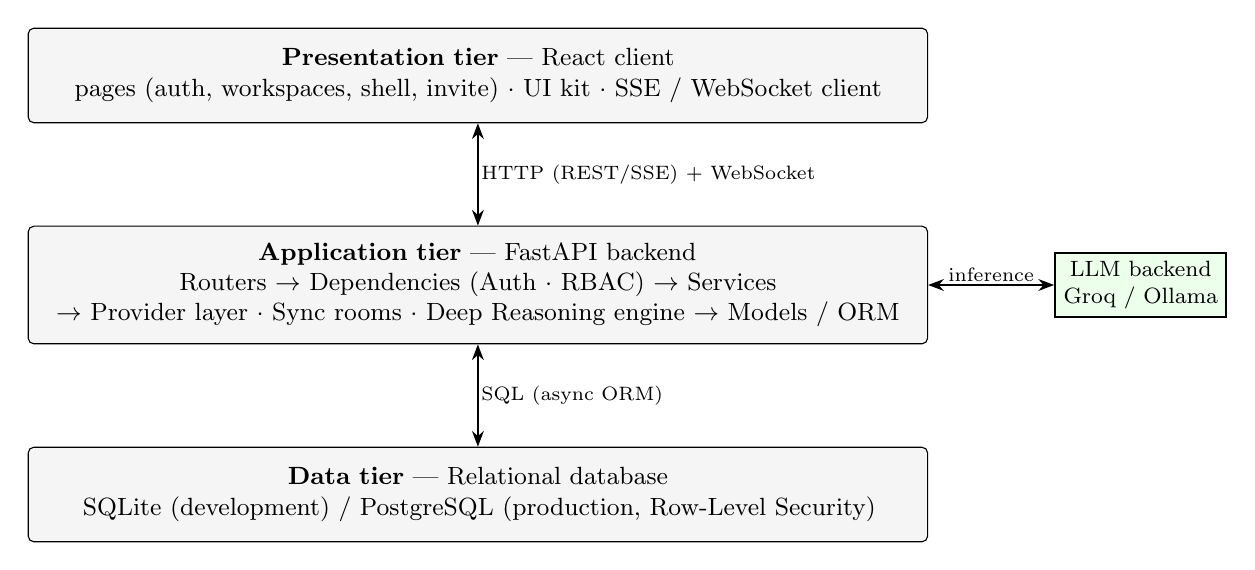
\begin{tikzpicture}
\node[tier, text width=11cm] (pres)
  {\textbf{Presentation tier} --- React client\\ pages (auth, workspaces, shell, invite) $\cdot$ UI kit $\cdot$ SSE / WebSocket client};
\node[tier, text width=11cm, below=13mm of pres] (app)
  {\textbf{Application tier} --- FastAPI backend\\ Routers $\rightarrow$ Dependencies (Auth $\cdot$ RBAC) $\rightarrow$ Services\\ $\rightarrow$ Provider layer $\cdot$ Sync rooms $\cdot$ Deep Reasoning engine $\rightarrow$ Models / ORM};
\node[tier, text width=11cm, below=13mm of app] (data)
  {\textbf{Data tier} --- Relational database\\ SQLite (development) / PostgreSQL (production, Row-Level Security)};
\node[ext, right=16mm of app] (llm) {LLM backend\\Groq / Ollama};
\draw[bi] (pres) -- node[lbl,right]{HTTP (REST/SSE) + WebSocket} (app);
\draw[bi] (app) -- node[lbl,right]{SQL (async ORM)} (data);
\draw[bi] (app) -- node[lbl,above]{inference} (llm);
\end{tikzpicture}
\end{adjustbox}
\caption{Three-tier architecture and backend layering}
\end{figure}

\section{Module Design}
Following a divide-and-conquer approach, the backend is decomposed into modules, each mapping to a concrete place in the codebase with one clear responsibility. The frontend modules mirror the surfaces: an API client and auth context, route-level page components (auth, workspaces, workspace shell, invite), and a shared UI-component kit.

\begingroup
\setlength{\parskip}{0pt}\renewcommand{\arraystretch}{1.32}\footnotesize
\begin{xltabular}{\textwidth}{>{\hsize=0.6635\hsize\raggedright\arraybackslash}X >{\hsize=1.5577\hsize\raggedright\arraybackslash}X >{\hsize=0.7788\hsize\raggedright\arraybackslash}X}
\caption{Module decomposition}\\
\toprule
\textbf{Module} & \textbf{Responsibility} & \textbf{Location} \\
\midrule\endfirsthead
\toprule
\textbf{Module} & \textbf{Responsibility} & \textbf{Location} \\
\midrule\endhead
\bottomrule\endfoot
Config & Typed settings from env/.env (DB URL, JWT, provider, URLs) & backend/api/config.py \\
DB / Session & Async engine, session-per-request, schema bootstrap, health ping & backend/api/db.py \\
Models & ORM entities + small domain helpers (role rank, expiry, UTC normalise) & backend/api/models.py \\
Security & bcrypt hashing, JWT encode/decode & backend/api/security.py \\
Deps (Auth + RBAC) & get\_current\_user, get\_membership, require\_role gate & backend/api/deps.py \\
Auth router & Register, login, /me & routers/auth.py \\
Workspaces router & Workspaces, invites, members, role patch & routers/workspaces.py \\
Provider layer & One streaming LLMProvider interface; stub/Groq/Ollama backends & backend/api/providers/* \\
Conversation service & Create conversations, persist nodes, drive the SSE send & routers/conversations.py \\
Fork service & O(1) fork; resolve history across branch boundaries; branch tree & services/fork.py \\
Sync / WS rooms & One in-memory room per workspace; presence; broadcast; per-client queues & ws/room.py \\
Prompt library & Save/search/tag prompts; usage counter & routers/prompts.py \\
Deep Reasoning engine & Recursive reason-reflect-synthesize loop; checkpointing; step/token events & backend/engine/* \\
Monitor service & Normalise engine events; meter tokens/rate vs thresholds & services/monitor.py \\
Run controller & Start/steer/kill; depth \& loop guards; RBAC-gated & routers/runs.py \\
History service & Replay a branch; export JSON/Markdown & routers/history.py \\
Permission policy & Owner-editable RBAC matrix; tool allowlist + approval & routers/permissions.py \\
\end{xltabular}
\endgroup

Dependencies point inward and downward; nothing in a lower layer imports a router. The two relationships that look bidirectional --- Conversation/Sync and Engine/Monitor --- are event-based (a service emits to the sync layer; it does not call back into the router), so there is no import cycle.

\begin{figure}[H]\centering
\begin{adjustbox}{max width=\textwidth}
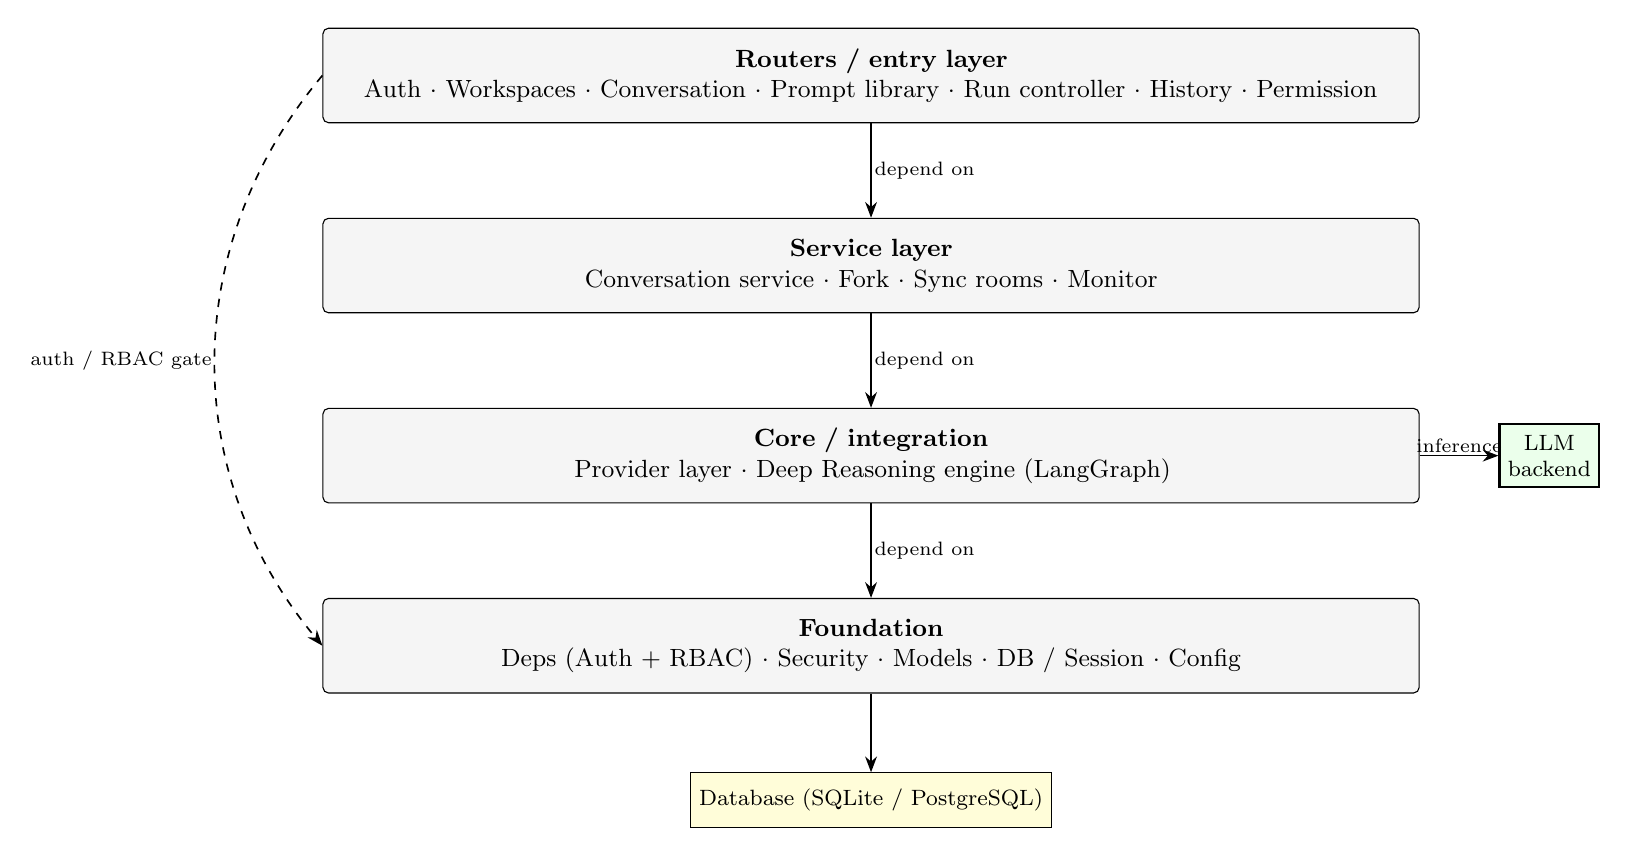
\begin{tikzpicture}
\node[tier, text width=13.5cm] (routers)
  {\textbf{Routers / entry layer}\\ Auth $\cdot$ Workspaces $\cdot$ Conversation $\cdot$ Prompt library $\cdot$ Run controller $\cdot$ History $\cdot$ Permission};
\node[tier, text width=13.5cm, below=12mm of routers] (services)
  {\textbf{Service layer}\\ Conversation service $\cdot$ Fork $\cdot$ Sync rooms $\cdot$ Monitor};
\node[tier, text width=13.5cm, below=12mm of services] (core)
  {\textbf{Core / integration}\\ Provider layer $\cdot$ Deep Reasoning engine (LangGraph)};
\node[tier, text width=13.5cm, below=12mm of core] (found)
  {\textbf{Foundation}\\ Deps (Auth + RBAC) $\cdot$ Security $\cdot$ Models $\cdot$ DB / Session $\cdot$ Config};
\node[ext, right=10mm of core] (llm) {LLM\\backend};
\node[store, below=10mm of found] (db) {Database (SQLite / PostgreSQL)};
\draw[fl] (routers) -- node[lbl,right]{depend on} (services);
\draw[fl] (services) -- node[lbl,right]{depend on} (core);
\draw[fl] (core) -- node[lbl,right]{depend on} (found);
\draw[fl] (core.east) -- node[lbl,above]{inference} (llm);
\draw[fl] (found) -- (db);
\draw[fl, dashed] (routers.west) to[bend right=40] node[lbl,left]{auth / RBAC gate} (found.west);
\end{tikzpicture}
\end{adjustbox}
\caption{Module dependency graph}
\end{figure}

\section{Data Flow Diagram}
The data-flow diagram is presented at three levels of information. Level 0 (context) shows the team member interacting with the Helix system and the external LLM backend. Level 1 expands the system into its principal processes --- authentication, workspace/RBAC, conversation/send, fork, prompt library, deep-reasoning, and monitor --- and their data stores. Level 2 details the Deep Reasoning process: escalate, reason-reflect-synthesize loop, metering, and kill/steer control.

\begin{figure}[H]\centering
\begin{adjustbox}{max width=\textwidth}
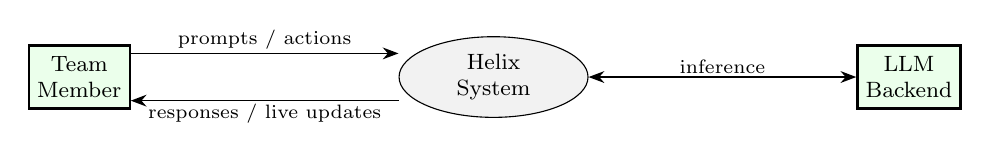
\begin{tikzpicture}
\node[ext] (m) {Team\\Member};
\node[proc, minimum width=24mm, right=34mm of m] (s) {Helix\\System};
\node[ext, right=34mm of s] (l) {LLM\\Backend};
\draw[fl] ([yshift=3mm]m.east) -- node[lbl,above]{prompts / actions} ([yshift=3mm]s.west);
\draw[fl] ([yshift=-3mm]s.west) -- node[lbl,below]{responses / live updates} ([yshift=-3mm]m.east);
\draw[bi] (s) -- node[lbl,above]{inference} (l);
\end{tikzpicture}
\end{adjustbox}
\caption{DFD Level 0 --- context diagram}
\end{figure}

\begin{figure}[H]\centering
\begin{adjustbox}{max width=\textwidth}
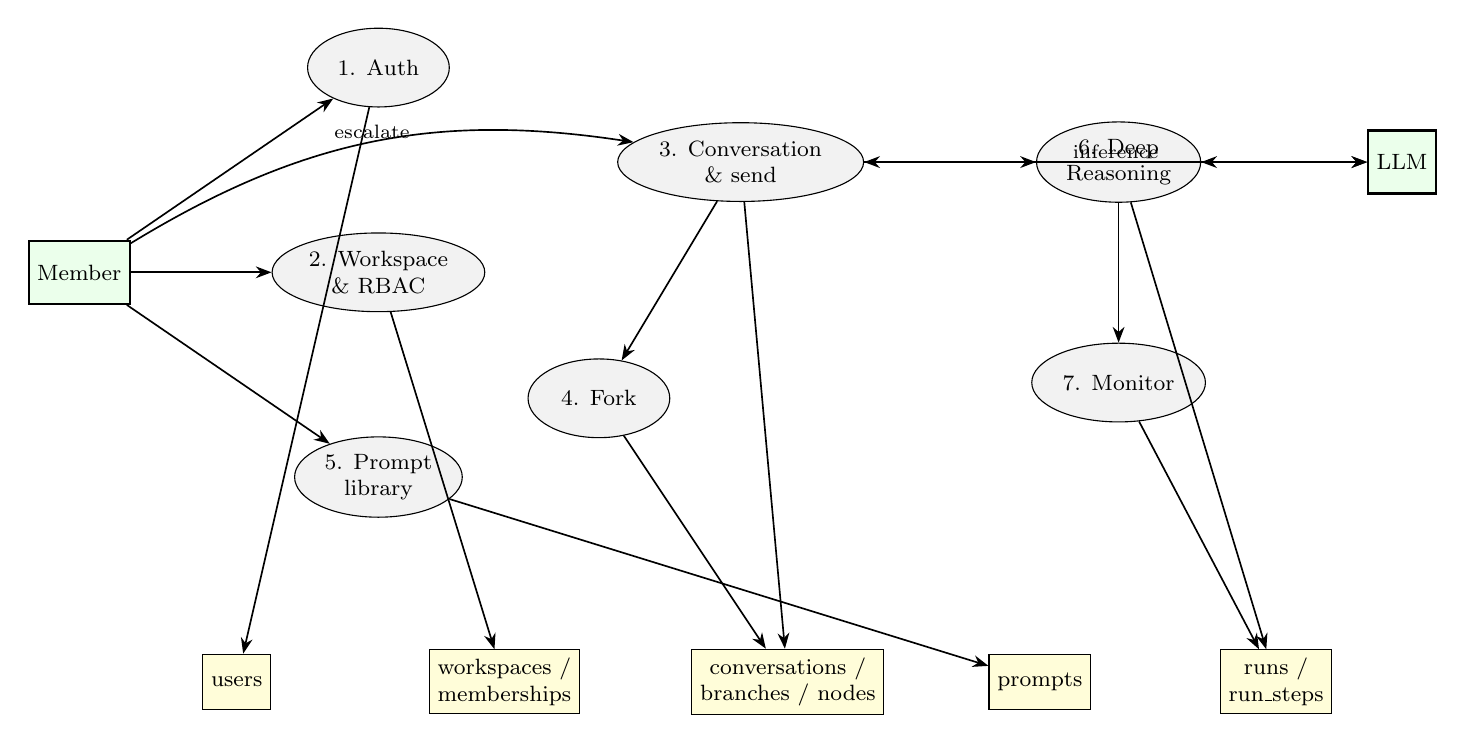
\begin{tikzpicture}
\node[ext] (m) at (0,3) {Member};
\node[proc] (p1) at (3.8,5.6) {1. Auth};
\node[proc] (p2) at (3.8,3) {2. Workspace\\\& RBAC};
\node[proc] (p5) at (3.8,0.4) {5. Prompt\\library};
\node[proc] (p3) at (8.4,4.4) {3. Conversation\\\& send};
\node[proc] (p4) at (6.6,1.4) {4. Fork};
\node[proc] (p6) at (13.2,4.4) {6. Deep\\Reasoning};
\node[proc] (p7) at (13.2,1.6) {7. Monitor};
\node[ext] (llm) at (16.8,4.4) {LLM};
\node[store] (d1) at (2.0,-2.2) {users};
\node[store] (d2) at (5.4,-2.2) {workspaces /\\memberships};
\node[store] (d3) at (9.0,-2.2) {conversations /\\branches / nodes};
\node[store] (d4) at (12.2,-2.2) {prompts};
\node[store] (d5) at (15.2,-2.2) {runs /\\run\_steps};
\draw[fl] (m) -- (p1);
\draw[fl] (m) -- (p2);
\draw[fl] (m) -- (p5);
\draw[fl] (m) to[bend left=20] node[lbl,above]{escalate} (p3);
\draw[fl] (p1) -- (d1);
\draw[fl] (p2) -- (d2);
\draw[fl] (p3) -- (d3);
\draw[fl] (p4) -- (d3);
\draw[fl] (p3) -- (p4);
\draw[fl] (p5) -- (d4);
\draw[bi] (p3) -- node[lbl,above]{inference} (llm);
\draw[bi] (p6) -- (llm);
\draw[fl] (p3) -- (p6);
\draw[fl] (p6) -- (p7);
\draw[fl] (p7) -- (d5);
\draw[fl] (p6) -- (d5);
\end{tikzpicture}
\end{adjustbox}
\caption{DFD Level 1 --- principal processes and data stores}
\end{figure}

\begin{figure}[H]\centering
\begin{adjustbox}{max width=\textwidth}
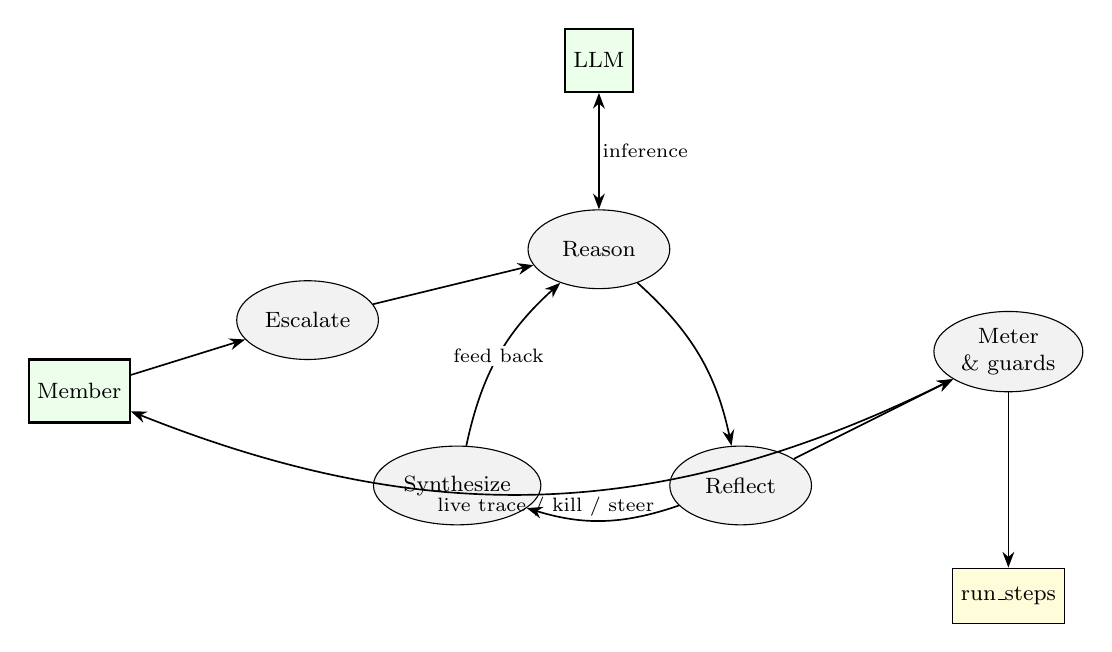
\begin{tikzpicture}
\node[ext] (m) at (0,0) {Member};
\node[proc] (esc) at (2.9,0.9) {Escalate};
\node[proc] (reason) at (6.6,1.8) {Reason};
\node[proc] (reflect) at (8.4,-1.2) {Reflect};
\node[proc] (synth) at (4.8,-1.2) {Synthesize};
\node[ext] (llm) at (6.6,4.2) {LLM};
\node[proc] (meter) at (11.8,0.5) {Meter\\\& guards};
\node[store] (steps) at (11.8,-2.6) {run\_steps};
\draw[fl] (m) -- (esc);
\draw[fl] (esc) -- (reason);
\draw[fl] (reason) to[bend left=18] (reflect);
\draw[fl] (reflect) to[bend left=18] (synth);
\draw[fl] (synth) to[bend left=18] node[card]{feed back} (reason);
\draw[bi] (reason) -- node[lbl,right]{inference} (llm);
\draw[fl] (reflect) -- (meter);
\draw[fl] (meter) -- (steps);
\draw[bi] (m) to[bend right=24] node[lbl,below]{live trace / kill / steer} (meter);
\end{tikzpicture}
\end{adjustbox}
\caption{DFD Level 2 --- Deep Reasoning process}
\end{figure}

\section{ER Diagram}
The entity-relationship model centres on the workspace as the tenant boundary. Users join workspaces through memberships (many-to-many, carrying the role); a workspace owns conversations, prompts, runs, permissions and invites; a conversation has branches; a branch groups append-only nodes and may be forked from another branch; a run emits ordered run-steps.

\begin{figure}[H]\centering
\begin{adjustbox}{max width=\textwidth}
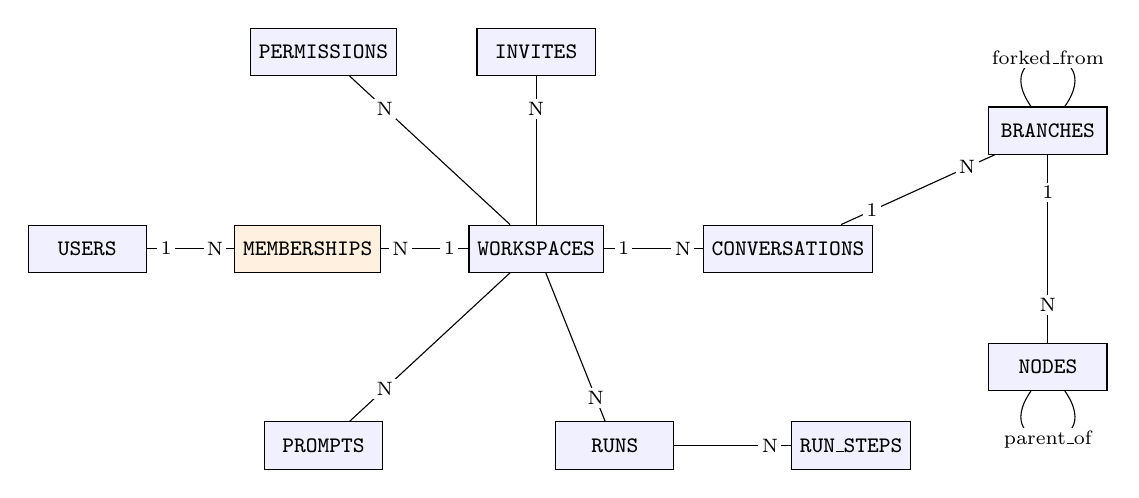
\begin{tikzpicture}
\node[ent] (users) at (0,0) {USERS};
\node[assoc] (mem) at (2.8,0) {MEMBERSHIPS};
\node[ent] (ws) at (5.7,0) {WORKSPACES};
\node[ent] (conv) at (8.9,0) {CONVERSATIONS};
\node[ent] (br) at (12.2,1.5) {BRANCHES};
\node[ent] (nodes) at (12.2,-1.5) {NODES};
\node[ent] (perm) at (3.0,2.5) {PERMISSIONS};
\node[ent] (inv) at (5.7,2.5) {INVITES};
\node[ent] (prompts) at (3.0,-2.5) {PROMPTS};
\node[ent] (runs) at (6.7,-2.5) {RUNS};
\node[ent] (steps) at (9.7,-2.5) {RUN\_STEPS};
\draw (users) -- node[card,pos=0.22]{1} node[card,pos=0.78]{N} (mem);
\draw (mem) -- node[card,pos=0.22]{N} node[card,pos=0.78]{1} (ws);
\draw (ws) -- node[card,pos=0.2]{1} node[card,pos=0.8]{N} (conv);
\draw (ws) -- node[card,pos=0.78]{N} (perm);
\draw (ws) -- node[card,pos=0.78]{N} (inv);
\draw (ws) -- node[card,pos=0.78]{N} (prompts);
\draw (ws) -- node[card,pos=0.84]{N} (runs);
\draw (conv) -- node[card,pos=0.2]{1} node[card,pos=0.82]{N} (br);
\draw (br) -- node[card,pos=0.2]{1} node[card,pos=0.8]{N} (nodes);
\draw (runs) -- node[card,pos=0.82]{N} (steps);
\draw (br) to[out=55,in=125,looseness=6] node[card]{forked\_from} (br);
\draw (nodes) to[out=-55,in=-125,looseness=6] node[card]{parent\_of} (nodes);
\end{tikzpicture}
\end{adjustbox}
\caption{Entity-Relationship diagram of the Helix schema}
\end{figure}

\section{Database Design}
The schema is shaped by five forces: strict multi-tenancy (every team-data row carries a workspace\_id), append-only server-ordered conversations (immutable nodes with a monotonic sequence number), structural branching (forks are pointers, not copies), policy-as-data (role permissions live in a table), and polyglot persistence (the same schema runs on SQLite for development and PostgreSQL for production).

\subsection{Table Design}
The principal tables and their structure are given below. Types are portable: on PostgreSQL UUID is native, timestamp is TIMESTAMPTZ and json is JSONB; on SQLite these are stored as TEXT. Enumerations are modelled as VARCHAR + CHECK.

\noindent\textbf{Table: users --- the account.}

\begingroup
\setlength{\parskip}{0pt}\renewcommand{\arraystretch}{1.32}\footnotesize
\begin{xltabular}{\textwidth}{>{\hsize=0.8000\hsize\raggedright\arraybackslash}X >{\hsize=0.6609\hsize\raggedright\arraybackslash}X >{\hsize=1.2174\hsize\raggedright\arraybackslash}X >{\hsize=1.3217\hsize\raggedright\arraybackslash}X}
\caption{users table}\\
\toprule
\textbf{Column} & \textbf{Type} & \textbf{Constraints} & \textbf{Description} \\
\midrule\endfirsthead
\toprule
\textbf{Column} & \textbf{Type} & \textbf{Constraints} & \textbf{Description} \\
\midrule\endhead
\bottomrule\endfoot
id & UUID & PK & Server-generated identity \\
email & VARCHAR(255) & UNIQUE, NOT NULL & Login identifier; case-insensitive \\
pw\_hash & VARCHAR(255) & NOT NULL & bcrypt hash of the password \\
created\_at & timestamp & NOT NULL, default now & Registration time \\
\end{xltabular}
\endgroup

\noindent\textbf{Table: workspaces --- the tenant.}

\begingroup
\setlength{\parskip}{0pt}\renewcommand{\arraystretch}{1.32}\footnotesize
\begin{xltabular}{\textwidth}{>{\hsize=0.8000\hsize\raggedright\arraybackslash}X >{\hsize=0.6609\hsize\raggedright\arraybackslash}X >{\hsize=1.2174\hsize\raggedright\arraybackslash}X >{\hsize=1.3217\hsize\raggedright\arraybackslash}X}
\caption{workspaces table}\\
\toprule
\textbf{Column} & \textbf{Type} & \textbf{Constraints} & \textbf{Description} \\
\midrule\endfirsthead
\toprule
\textbf{Column} & \textbf{Type} & \textbf{Constraints} & \textbf{Description} \\
\midrule\endhead
\bottomrule\endfoot
id & UUID & PK & Tenant boundary key (on all owned rows) \\
name & VARCHAR(120) & NOT NULL & Display name \\
owner\_id & UUID & FK $\rightarrow$ users.id, NOT NULL & The founding Owner \\
created\_at & timestamp & NOT NULL, default now & Creation time \\
\end{xltabular}
\endgroup

\noindent\textbf{Table: memberships --- user-to-workspace association carrying the role.}

\begingroup
\setlength{\parskip}{0pt}\renewcommand{\arraystretch}{1.32}\footnotesize
\begin{xltabular}{\textwidth}{>{\hsize=0.8000\hsize\raggedright\arraybackslash}X >{\hsize=0.6609\hsize\raggedright\arraybackslash}X >{\hsize=1.2174\hsize\raggedright\arraybackslash}X >{\hsize=1.3217\hsize\raggedright\arraybackslash}X}
\caption{memberships table}\\
\toprule
\textbf{Column} & \textbf{Type} & \textbf{Constraints} & \textbf{Description} \\
\midrule\endfirsthead
\toprule
\textbf{Column} & \textbf{Type} & \textbf{Constraints} & \textbf{Description} \\
\midrule\endhead
\bottomrule\endfoot
id & UUID & PK & Surrogate identity \\
user\_id & UUID & FK $\rightarrow$ users.id, NOT NULL & Member \\
workspace\_id & UUID & FK $\rightarrow$ workspaces.id, NOT NULL & Tenant \\
role & VARCHAR(16) & NOT NULL, CHECK in \{owner, collaborator, observer\} & Authorisation role \\
joined\_at & timestamp & NOT NULL, default now & When they joined \\
\end{xltabular}
\endgroup

\noindent\textbf{Table: conversations --- a thread within a workspace, shared or private.}

\begingroup
\setlength{\parskip}{0pt}\renewcommand{\arraystretch}{1.32}\footnotesize
\begin{xltabular}{\textwidth}{>{\hsize=0.8000\hsize\raggedright\arraybackslash}X >{\hsize=0.6609\hsize\raggedright\arraybackslash}X >{\hsize=1.2174\hsize\raggedright\arraybackslash}X >{\hsize=1.3217\hsize\raggedright\arraybackslash}X}
\caption{conversations table}\\
\toprule
\textbf{Column} & \textbf{Type} & \textbf{Constraints} & \textbf{Description} \\
\midrule\endfirsthead
\toprule
\textbf{Column} & \textbf{Type} & \textbf{Constraints} & \textbf{Description} \\
\midrule\endhead
\bottomrule\endfoot
id & UUID & PK & Conversation identity \\
workspace\_id & UUID & FK $\rightarrow$ workspaces.id, NOT NULL & Tenant scope \\
author\_id & UUID & FK $\rightarrow$ users.id, NOT NULL & Creator (only viewer if private) \\
title & VARCHAR(200) & NOT NULL & Display title \\
visibility & VARCHAR(8) & NOT NULL, CHECK in \{shared, private\} & Access mode \\
default\_branch\_id & UUID & FK $\rightarrow$ branches.id (deferrable) & Root branch \\
created\_at & timestamp & NOT NULL, default now & Creation time \\
\end{xltabular}
\endgroup

\noindent\textbf{Table: branches --- a line in the conversation tree; the table that makes forks O(1).}

\begingroup
\setlength{\parskip}{0pt}\renewcommand{\arraystretch}{1.32}\footnotesize
\begin{xltabular}{\textwidth}{>{\hsize=0.8000\hsize\raggedright\arraybackslash}X >{\hsize=0.6609\hsize\raggedright\arraybackslash}X >{\hsize=1.2174\hsize\raggedright\arraybackslash}X >{\hsize=1.3217\hsize\raggedright\arraybackslash}X}
\caption{branches table}\\
\toprule
\textbf{Column} & \textbf{Type} & \textbf{Constraints} & \textbf{Description} \\
\midrule\endfirsthead
\toprule
\textbf{Column} & \textbf{Type} & \textbf{Constraints} & \textbf{Description} \\
\midrule\endhead
\bottomrule\endfoot
id & UUID & PK & Branch identity \\
conversation\_id & UUID & FK $\rightarrow$ conversations.id, NOT NULL & Owning conversation \\
name & VARCHAR(120) & NOT NULL & Branch label \\
parent\_branch\_id & UUID & FK $\rightarrow$ branches.id, NULL for root & Lineage link \\
fork\_node\_id & UUID & FK $\rightarrow$ nodes.id, NULL for root & Divergence point \\
head\_node\_id & UUID & FK $\rightarrow$ nodes.id, NULL until first message & Cached tip \\
engine\_thread\_id & VARCHAR(64) & NULL & LangGraph checkpoint id (deep-reasoning branches) \\
created\_at & timestamp & NOT NULL, default now & Creation time \\
\end{xltabular}
\endgroup

\noindent\textbf{Table: nodes --- the append-only, immutable message units.}

\begingroup
\setlength{\parskip}{0pt}\renewcommand{\arraystretch}{1.32}\footnotesize
\begin{xltabular}{\textwidth}{>{\hsize=0.8000\hsize\raggedright\arraybackslash}X >{\hsize=0.6609\hsize\raggedright\arraybackslash}X >{\hsize=1.2174\hsize\raggedright\arraybackslash}X >{\hsize=1.3217\hsize\raggedright\arraybackslash}X}
\caption{nodes table}\\
\toprule
\textbf{Column} & \textbf{Type} & \textbf{Constraints} & \textbf{Description} \\
\midrule\endfirsthead
\toprule
\textbf{Column} & \textbf{Type} & \textbf{Constraints} & \textbf{Description} \\
\midrule\endhead
\bottomrule\endfoot
id & UUID & PK & Node identity \\
branch\_id & UUID & FK $\rightarrow$ branches.id, NOT NULL & Branch written on \\
parent\_id & UUID & FK $\rightarrow$ nodes.id, NULL at root & Previous node (fork spine) \\
seq & INTEGER & NOT NULL & Monotonic order within branch \\
author\_id & UUID & FK $\rightarrow$ users.id, NULL for assistant/system & Who sent it \\
role & VARCHAR(10) & NOT NULL, CHECK in \{user, assistant, system\} & Message role \\
content & json & NOT NULL & Message payload \\
token\_count & INTEGER & NOT NULL, default 0 & Cached token size \\
created\_at & timestamp & NOT NULL, default now & Write time \\
\end{xltabular}
\endgroup

\noindent\textbf{Table: prompts --- the shared, searchable prompt library.}

\begingroup
\setlength{\parskip}{0pt}\renewcommand{\arraystretch}{1.32}\footnotesize
\begin{xltabular}{\textwidth}{>{\hsize=0.8000\hsize\raggedright\arraybackslash}X >{\hsize=0.6609\hsize\raggedright\arraybackslash}X >{\hsize=1.2174\hsize\raggedright\arraybackslash}X >{\hsize=1.3217\hsize\raggedright\arraybackslash}X}
\caption{prompts table}\\
\toprule
\textbf{Column} & \textbf{Type} & \textbf{Constraints} & \textbf{Description} \\
\midrule\endfirsthead
\toprule
\textbf{Column} & \textbf{Type} & \textbf{Constraints} & \textbf{Description} \\
\midrule\endhead
\bottomrule\endfoot
id & UUID & PK & Prompt identity \\
workspace\_id & UUID & FK $\rightarrow$ workspaces.id, NOT NULL & Tenant scope \\
author\_id & UUID & FK $\rightarrow$ users.id, NOT NULL & Who saved it \\
title & VARCHAR(200) & NOT NULL & Short label \\
body & TEXT & NOT NULL & The prompt text \\
tags & json & NOT NULL, default [] & String tag array \\
used\_count & INTEGER & NOT NULL, default 0 & Times inserted (what-works signal) \\
created\_at & timestamp & NOT NULL, default now & Saved at \\
\end{xltabular}
\endgroup

\noindent\textbf{Table: runs --- a Deep-Reasoning escalation of a branch.}

\begingroup
\setlength{\parskip}{0pt}\renewcommand{\arraystretch}{1.32}\footnotesize
\begin{xltabular}{\textwidth}{>{\hsize=0.8000\hsize\raggedright\arraybackslash}X >{\hsize=0.6609\hsize\raggedright\arraybackslash}X >{\hsize=1.2174\hsize\raggedright\arraybackslash}X >{\hsize=1.3217\hsize\raggedright\arraybackslash}X}
\caption{runs table}\\
\toprule
\textbf{Column} & \textbf{Type} & \textbf{Constraints} & \textbf{Description} \\
\midrule\endfirsthead
\toprule
\textbf{Column} & \textbf{Type} & \textbf{Constraints} & \textbf{Description} \\
\midrule\endhead
\bottomrule\endfoot
id & UUID & PK & Run identity \\
workspace\_id & UUID & FK $\rightarrow$ workspaces.id, NOT NULL & Tenant scope \\
conversation\_id & UUID & FK $\rightarrow$ conversations.id, NOT NULL & Source conversation \\
branch\_id & UUID & FK $\rightarrow$ branches.id, NOT NULL & Branch reasoned on \\
status & VARCHAR(10) & CHECK in \{running, paused, done, killed, error\} & Lifecycle state \\
provider & VARCHAR(16) & NOT NULL & LLM backend used \\
model & VARCHAR(64) & NULL & Concrete model name \\
stop\_reason & VARCHAR(32) & NULL & Why it halted \\
started\_at & timestamp & NOT NULL, default now & Start \\
ended\_at & timestamp & NULL & End (null while live) \\
\end{xltabular}
\endgroup

\noindent\textbf{Table: run\_steps --- the persisted reasoning trace (one row per engine transition).}

\begingroup
\setlength{\parskip}{0pt}\renewcommand{\arraystretch}{1.32}\footnotesize
\begin{xltabular}{\textwidth}{>{\hsize=0.8000\hsize\raggedright\arraybackslash}X >{\hsize=0.6609\hsize\raggedright\arraybackslash}X >{\hsize=1.2174\hsize\raggedright\arraybackslash}X >{\hsize=1.3217\hsize\raggedright\arraybackslash}X}
\caption{run\_steps table}\\
\toprule
\textbf{Column} & \textbf{Type} & \textbf{Constraints} & \textbf{Description} \\
\midrule\endfirsthead
\toprule
\textbf{Column} & \textbf{Type} & \textbf{Constraints} & \textbf{Description} \\
\midrule\endhead
\bottomrule\endfoot
id & UUID & PK & Step identity \\
run\_id & UUID & FK $\rightarrow$ runs.id, NOT NULL & Owning run \\
idx & INTEGER & NOT NULL & Ordinal within the run \\
node & VARCHAR(24) & NOT NULL & Engine node (reason/reflect/synthesize) \\
payload & json & NOT NULL & Step event (thought, energy, depth, readings) \\
token\_count & INTEGER & NOT NULL, default 0 & Tokens used this step \\
latency\_ms & INTEGER & NOT NULL, default 0 & Step duration \\
created\_at & timestamp & NOT NULL, default now & Emitted at \\
\end{xltabular}
\endgroup

\noindent\textbf{Table: permissions --- RBAC as data (per-workspace, per-role, per-action policy).}

\begingroup
\setlength{\parskip}{0pt}\renewcommand{\arraystretch}{1.32}\footnotesize
\begin{xltabular}{\textwidth}{>{\hsize=0.8000\hsize\raggedright\arraybackslash}X >{\hsize=0.6609\hsize\raggedright\arraybackslash}X >{\hsize=1.2174\hsize\raggedright\arraybackslash}X >{\hsize=1.3217\hsize\raggedright\arraybackslash}X}
\caption{permissions table}\\
\toprule
\textbf{Column} & \textbf{Type} & \textbf{Constraints} & \textbf{Description} \\
\midrule\endfirsthead
\toprule
\textbf{Column} & \textbf{Type} & \textbf{Constraints} & \textbf{Description} \\
\midrule\endhead
\bottomrule\endfoot
workspace\_id & UUID & PK (composite), FK $\rightarrow$ workspaces.id & Tenant scope \\
role & VARCHAR(16) & PK (composite), CHECK in \{owner, collaborator, observer\} & Role \\
action & VARCHAR(40) & PK (composite) & Action key (e.g. message.send) \\
allowed & BOOLEAN & NOT NULL & Whether the role may perform the action \\
\end{xltabular}
\endgroup

The invites table (token PK, workspace\_id, created\_by, role, expires\_at, created\_at) stores opaque, expiring onboarding links and is omitted here for brevity.

\subsection{Data Integrity and Constraints}
\begin{itemize}
  \item Primary keys are server-generated UUID strings, except invites.token (the secret itself) and the composite PK of permissions.
  \item Uniqueness: users.email; memberships(user\_id, workspace\_id); nodes(branch\_id, seq); run\_steps(run\_id, idx).
  \item Foreign keys use ON DELETE CASCADE down ownership chains (deleting a workspace removes its conversations, branches, nodes, prompts, runs, steps, memberships, permissions and invites) and ON DELETE SET NULL for soft links (nodes.author\_id when a user is removed but their messages remain).
  \item A deferrable constraint links conversations.default\_branch\_id and branches.conversation\_id, satisfied within the create-conversation transaction.
  \item Not-null discipline: every tenant row's workspace\_id is NOT NULL --- there is no unscoped resource.
  \item Visibility is enforced on every read: a conversation is visible where workspace\_id = :wid AND (visibility = 'shared' OR author\_id = :uid).
  \item On production PostgreSQL, Row-Level Security policies on every tenant-scoped table constrain access to the active workspace, set per request via a session variable --- so even a coding mistake cannot leak across tenants.
\end{itemize}

\subsection{Data Dictionary}
Domains and enumerations --- centralised value sets, each enforced by a CHECK constraint (portable across SQLite and PostgreSQL):

\begingroup
\setlength{\parskip}{0pt}\renewcommand{\arraystretch}{1.32}\footnotesize
\begin{xltabular}{\textwidth}{>{\hsize=0.5405\hsize\raggedright\arraybackslash}X >{\hsize=1.4595\hsize\raggedright\arraybackslash}X}
\caption{Domains and enumerations}\\
\toprule
\textbf{Domain} & \textbf{Permitted values} \\
\midrule\endfirsthead
\toprule
\textbf{Domain} & \textbf{Permitted values} \\
\midrule\endhead
\bottomrule\endfoot
role & owner, collaborator, observer (owner > collaborator > observer) \\
visibility & shared, private \\
node.role & user, assistant, system \\
run.status & running, paused, done, killed, error \\
run.stop\_reason & converged, budget, depth\_guard, loop\_guard, killed, error \\
provider & stub, groq, ollama \\
\end{xltabular}
\endgroup

RBAC policy matrix --- the permissions table is seeded on workspace creation from the following default matrix (the Owner may later edit it):

\begingroup
\setlength{\parskip}{0pt}\renewcommand{\arraystretch}{1.32}\footnotesize
\begin{xltabular}{\textwidth}{>{\hsize=1.7778\hsize\raggedright\arraybackslash}X >{\hsize=0.6667\hsize\centering\arraybackslash}X >{\hsize=0.8889\hsize\centering\arraybackslash}X >{\hsize=0.6667\hsize\centering\arraybackslash}X}
\caption{Default RBAC policy matrix}\\
\toprule
\textbf{Action} & \textbf{Owner} & \textbf{Collaborator} & \textbf{Observer} \\
\midrule\endfirsthead
\toprule
\textbf{Action} & \textbf{Owner} & \textbf{Collaborator} & \textbf{Observer} \\
\midrule\endhead
\bottomrule\endfoot
conversation.read / replay & Yes & Yes & Yes \\
message.send & Yes & Yes & No \\
branch.fork & Yes & Yes & No \\
prompt.write (save/edit) & Yes & Yes & No \\
run.escalate (Deep Reasoning) & Yes & Yes & No \\
run.steer / run.kill & Yes & Yes & No \\
member.invite / member.role & Yes & No & No \\
permission.edit & Yes & No & No \\
\end{xltabular}
\endgroup

\section{Interface and Procedural Design}
\subsection{User Interface Design}
The interface follows one governing principle --- ornament at the edges, clarity at the centre. The aesthetic (``Alchemical Noir'': a near-black canvas, antique-gold line-work, arcane-violet accents) lives in brand moments such as authentication, loaders and the Deep Reasoning monitor, while the working surfaces where members read and write stay calm, legible and high-contrast. The product comprises eight primary screens. Rough wireframes are given below; final screenshots are to be inserted in their reserved spaces.

\noindent\textbf{(1) Authentication (Login / Register)}

A ceremonial entry: the brand mark over a slow golden-spiral drift and a single calm card with email and password. A single primary action; errors appear inline beneath the field; the DNA-helix loader replaces the button label while authenticating.

\begin{figure}[H]\centering
\begin{lstlisting}
+----------------------------------------------+
|        (slow golden-spiral drift)            |
|              H E L I X                        |
|   "where a team's reasoning converges"        |
|   +--------------------------------------+   |
|   | Sign in                              |   |
|   | Email    [ ................. ]        |   |
|   | Password [ ................. ]        |   |
|   |            [ Enter the atelier ]      |   |
|   | New here?  Create an account ->      |   |
|   +--------------------------------------+   |
+----------------------------------------------+
\end{lstlisting}
\caption{UI --- Authentication (Login / Register)}
\end{figure}

\noindent\textbf{(2) Invite Accept}

A focused hand-off showing who invited you, into which workspace, and with which role, with one decisive Accept action. The invite preview needs no login; an expired token shows a calm empty state.

\begin{figure}[H]\centering
\begin{lstlisting}
+--------------------------------------+
|   You've been invited to join        |
|        (oo) rag-quality              |
|   as a  Collaborator                 |
|        [ Accept & enter ]            |
|         Not now                      |
+--------------------------------------+
\end{lstlisting}
\caption{UI --- Invite Accept}
\end{figure}

\noindent\textbf{(3) Workspaces - Radial Launcher}

A circular navigation wheel: workspace sigils orbit the central mark. Hovering a node shows its name, role glyph, member count and last-active; '+ new' opens a create modal. A plain list is the fallback past about eight workspaces.

\begin{figure}[H]\centering
\begin{lstlisting}
            rag-quality     infra-notes
         design       (you)        research
            onboarding         + new
   hover -> name, role, members, last-active
\end{lstlisting}
\caption{UI --- Workspaces - Radial Launcher}
\end{figure}

\noindent\textbf{(4) Workspace Shell - Collaboration View}

The everyday surface, split on the golden ratio: a narrow rail (conversations + branch tree), a wide thread, and presence along the top. Visibility sigils mark shared vs private; Fork sits at the thread head; the composer carries Send and a Deep Reason action.

\begin{figure}[H]\centering
\begin{lstlisting}
+-------------------------------------------------------------+
| Helix . rag-quality      (.)Aria (.)Ben (.)Cara  [gear]     |
+--------------+----------------------------------------------+
| CONVERSATIONS|  retrieval staleness            [ Fork ]     |
|  (oo)retrieval| Aria  Why is retrieval stale?               |
|  (oo)chunking | AI    Because the cache TTL... |            |
|  (lock)notes  |                                              |
| BRANCH TREE   |                                              |
|  o main       |                                              |
|  +-o chunk-v2 | [ type a prompt...    ] [Send] [ Deep ]      |
+--------------+----------------------------------------------+
\end{lstlisting}
\caption{UI --- Workspace Shell - Collaboration View}
\end{figure}

\noindent\textbf{(5) Branch Tree}

The double-helix made navigable - lineage as a gold spine with helix nodes. Selecting a node opens that branch; 'Fork here' creates a child; the active branch is bright gold; large trees pan and zoom.

\begin{figure}[H]\centering
\begin{lstlisting}
  o main ------o------o------o (head)
              |
              +--o chunk-v2 ---o---o (head)
                      |
                      +--o chunk-v2-rerank --o (head)
\end{lstlisting}
\caption{UI --- Branch Tree}
\end{figure}

\noindent\textbf{(6) Prompt Library}

The team's record of working prompts - calm, searchable and clean. Search filters title/body/tags live; Insert drops the body into the active composer; a use-count is the social proof of what works.

\begin{figure}[H]\centering
\begin{lstlisting}
+--------------------------------------------------------+
| Prompt Library     [ search... ]  tags: [rag][eval]    |
+--------------------------------------------------------+
| failure-classification     by Cara . used 7x  [Insert] |
|   "Given these error logs, classify each..."  #rag      |
| chunk-size sweep           by Ben  . used 3x  [Insert] |
|   "Compare retrieval quality across sizes..." #retr    |
+--------------------------------------------------------+
             [ + Save current prompt ]
\end{lstlisting}
\caption{UI --- Prompt Library}
\end{figure}

\noindent\textbf{(7) Deep Reasoning Monitor - the Ouroboros}

The signature screen: the recursive engine drawn as an ouroboros. Reason, reflect and synthesise sit on a ring traced once per loop; concentric rings show recursion depth; a step trace lists each transition; energy, depth, loop-guard and a budget meter sit below. Kill is an unmissable control; Steer pauses and resumes with guidance. For an Observer, Steer/Kill are absent and the screen reads 'Watching'.

\begin{figure}[H]\centering
\begin{lstlisting}
+-------------------------------------------------------------+
| Deep Reasoning . run #a3f  running   [ Steer ] [ Kill ]     |
+-------------------------------+-----------------------------+
|       THE OUROBOROS           |  STEP TRACE                 |
|        reason (o)             |  #1 reason  d1 120ms 410tok |
|       /        \              |  #2 reflect d1  95ms 220tok |
|  synth (o)    (o) reflect     |  #3 reason  d2 140ms 500tok<|
|       (depth rings)           |  #4 reflect d2  88ms 210tok |
+-------------------------------+-----------------------------+
| energy ####_ 0.62  depth 2/6  loop-guard 3/8                |
| budget ########_ 85%  ! threshold  (4.3k / 5k tokens)       |
+-------------------------------------------------------------+
\end{lstlisting}
\caption{UI --- Deep Reasoning Monitor - the Ouroboros}
\end{figure}

\noindent\textbf{(8) Replay \& Export}

Turning a run into a kept artifact. A scrubber steps through any branch or run node-by-node (the ring re-traces for runs); export offers JSON or Markdown for the current scope.

\begin{figure}[H]\centering
\begin{lstlisting}
+--------------------------------------------------------+
| Replay . chunk-v2   |<< < ||  > >>    step 6 / 14       |
|  (the thread / ring re-animates to this point)         |
|  Export: [ JSON ]  [ Markdown ]      scope: this       |
+--------------------------------------------------------+
\end{lstlisting}
\caption{UI --- Replay \& Export}
\end{figure}

Reports / Exports. Helix generates two kept-artifact reports. The Conversation/Run export takes a conversation or run as input (with a scope selector) and outputs an ordered JSON or Markdown document of nodes/steps. The Deep Reasoning run summary outputs the run's status, stop reason, total tokens, depth reached, and the ordered step trace. Reserved space for these report screens is shown below.

\begin{figure}[H]\centering
\fbox{\begin{minipage}[c][3cm][c]{0.92\textwidth}\centering
\textit{\textcolor{gray}{[ Space reserved for diagram --- insert here ]}}
\end{minipage}}
\caption{Report --- Conversation / Run export (JSON / Markdown)}
\end{figure}

\begin{figure}[H]\centering
\fbox{\begin{minipage}[c][3cm][c]{0.92\textwidth}\centering
\textit{\textcolor{gray}{[ Space reserved for diagram --- insert here ]}}
\end{minipage}}
\caption{Report --- Deep Reasoning run summary}
\end{figure}

\section{Algorithm Design}
This section specifies the non-trivial algorithms at the heart of Helix --- each with its purpose, pseudocode, complexity and a note on correctness or termination.

\subsection{A1 --- O(1) Fork and Cross-Branch History Resolution}
A fork must be instant regardless of conversation length, so it copies no history; the cost is shifted to a read-time walk up the parent\_id spine, which transparently crosses branch boundaries (Git-style structural sharing).

\begin{lstlisting}
FUNCTION fork(cid, N, name, is_deep_reasoning):
    B <- new Branch { conversation_id=cid, name=name,
        parent_branch_id=N.branch_id,   # lineage
        fork_node_id=N.id,              # divergence point
        head_node_id=N.id, engine_thread_id=NULL }
    IF is_deep_reasoning AND branch_of(N).engine_thread_id != NULL:
        B.engine_thread_id <- copy_checkpoint(branch_of(N).engine_thread_id)
    persist(B)            # exactly ONE row inserted
    RETURN B

FUNCTION resolve_history(B):
    out <- empty list ; node <- B.head_node   # O(1) via cached head
    WHILE node != NULL:
        out.prepend(node)
        node <- node.parent          # follows parent_id ACROSS branches
    RETURN out
\end{lstlisting}

Complexity: fork is O(1) writes (one row; plus an O(1) checkpoint-pointer copy for reasoning branches), independent of conversation length; history resolution is O(n) in the number of nodes on the path. Correctness: nodes are immutable and parent\_id forms a tree, so a branch merely names a tip and a fork point --- no existing node is mutated. The read path, not the write, is where correctness must be tested hardest (crossing the branch boundary at the fork node).

\subsection{A2 --- Two-Stage RBAC Authorization}
Authorisation is a fast coarse gate (role rank) followed, where needed, by a fine-grained, data-driven policy lookup. The membership lookup doubles as the tenant-isolation check.

\begin{lstlisting}
ROLE_RANK = { observer:0, collaborator:1, owner:2 }

FUNCTION require_role(user, wid, min_role):      # coarse gate
    m <- membership(user.id, wid)
    IF m = NULL:  RAISE 404 not_found   # non-member: hide tenant
    IF ROLE_RANK[m.role] < ROLE_RANK[min_role]: RAISE 403 forbidden
    RETURN m

FUNCTION can(wid, role, action):                 # policy-as-data
    row <- permissions[wid, role, action]
    IF row != NULL: RETURN row.allowed
    RETURN DEFAULT_MATRIX[role, action]          # default-deny
\end{lstlisting}

Complexity: O(1) --- two point lookups on indexed/PK columns. A non-member fails before any resource is loaded, and the response is 404 (not 403) so the system never discloses that the workspace exists. Any action absent from both the policy and the default matrix resolves to not-allowed (default-deny).

\subsection{A3 --- Recursive Deep Reasoning Loop}
The agentic core: reason, reflect, synthesize, feeding each synthesis back as the next thought (the ouroboros), looping until it converges or any one of four independent guards halts it. A step event is emitted per transition for the live monitor and the persisted trace.

\begin{lstlisting}
FUNCTION deep_reason(run, prompt, config):
    state <- { thought:prompt, depth:0, loops:0, tokens:0, energy:1.0 }
    WHILE TRUE:
        IF run.kill_requested:                 RETURN halt('killed')
        IF state.tokens >= config.token_budget: RETURN halt('budget')
        IF state.depth  >= config.max_depth:    RETURN halt('depth_guard')
        IF state.loops  >= config.loop_guard:   RETURN halt('loop_guard')
        IF run.steer_pending: state <- inject(state, await_steer(run))
        reasoning <- LLM.reason(state.thought)         ; emit('reason')
        critique  <- LLM.reflect(reasoning)            ; emit('reflect')
        synthesis <- LLM.synthesize(reasoning,critique); emit('synthesize')
        state.tokens += tokens_used(...) ; emit_budget(...)
        state.energy = decay(state.energy)   # strictly decreasing
        IF converged(synthesis) OR state.energy < config.energy_floor:
            RETURN complete(run, synthesis, 'converged')
        state.thought = synthesis ; state.depth += 1 ; state.loops += 1
\end{lstlisting}

Complexity: O(S) reasoning iterations, bounded above by min(max\_depth, loop\_guard, token\_budget / per\_step\_tokens). Termination is guaranteed by four independent halts (kill, budget, depth, loop) and a strictly decreasing energy that hits energy\_floor --- no input can produce an unbounded loop. Because the loop only checks for human input at a step boundary, injected guidance never corrupts mid-transition state.

\subsection{A4--A7 --- Supporting Algorithms}
\begin{itemize}
  \item A4 --- Budget metering and threshold alerting. Accumulates per-step tokens, drives the budget meter, raises a one-shot alert at the threshold (an alerted latch prevents spam), and requests a cooperative halt at the next boundary when the budget is reached. O(1) amortised per step.
  \item A5 --- Real-time fan-out with authoritative ordering. A monotonic seq is assigned inside the write transaction (server owns order); broadcast enqueues to per-client bounded queues non-blockingly, so a slow consumer fills only its own queue and is dropped without head-of-line blocking. Clients render by seq, not arrival. O(C) enqueues per event.
  \item A6 --- Prompt library search and ranking. Full-text (GIN) candidate retrieval filtered by tags, ranked by text relevance then used\_count (the team's what-works signal) then recency; degrades to a LIKE scan on SQLite. Sub-linear retrieval + O(k log k) ranking.
  \item A7 --- Invite token lifecycle. A 256-bit url-safe random token is the primary key; acceptance is a PK lookup with UTC-normalised expiry checking, idempotent re-accept, and not-found for expired tokens to avoid leaking workspace existence. O(1).
\end{itemize}

\begingroup
\setlength{\parskip}{0pt}\renewcommand{\arraystretch}{1.32}\footnotesize
\begin{xltabular}{\textwidth}{>{\hsize=0.3279\hsize\raggedright\arraybackslash}X >{\hsize=1.3934\hsize\raggedright\arraybackslash}X >{\hsize=0.9426\hsize\raggedright\arraybackslash}X >{\hsize=0.7787\hsize\raggedright\arraybackslash}X >{\hsize=1.5574\hsize\raggedright\arraybackslash}X}
\caption{Algorithm complexity summary}\\
\toprule
\textbf{\#} & \textbf{Algorithm} & \textbf{Time} & \textbf{Space} & \textbf{Key guarantee} \\
\midrule\endfirsthead
\toprule
\textbf{\#} & \textbf{Algorithm} & \textbf{Time} & \textbf{Space} & \textbf{Key guarantee} \\
\midrule\endhead
\bottomrule\endfoot
A1 & Fork (write) & O(1) & O(1) & No history copied \\
A1 & History resolution (read) & O(n) & O(n) & Correct cross-branch walk \\
A2 & RBAC authorization & O(1) & O(1) & Default-deny; tenant-isolating \\
A3 & Deep Reasoning loop & O(S) & O(1) state & Guaranteed termination (4 guards + energy) \\
A4 & Budget metering & O(1)/step & O(k) window & One-shot alert; cooperative halt \\
A5 & Fan-out + ordering & O(C)/event & O(C) queues & Total order by seq; no HOL blocking \\
A6 & Library search & sub-linear + O(k log k) & O(k) & Relevance then proven usefulness \\
A7 & Invite lifecycle & O(1) & O(1) & Unguessable, expiring, idempotent \\
\end{xltabular}
\endgroup

\end{document}